This chapter addresses the modules responsible for allowing users to
invoke the framework through a standard Python script and a high-level
YAML file. It also addresses the generative AI modules that can assist a
user in building a scenario. These modules are depicted in
\autoref{fig:scenarios-simple} below, with a more detailed diagram
located in \autoref{appendix-a} as
\autoref{fig:architecture-full-a}.

\begin{figure}[htbp]
\centering
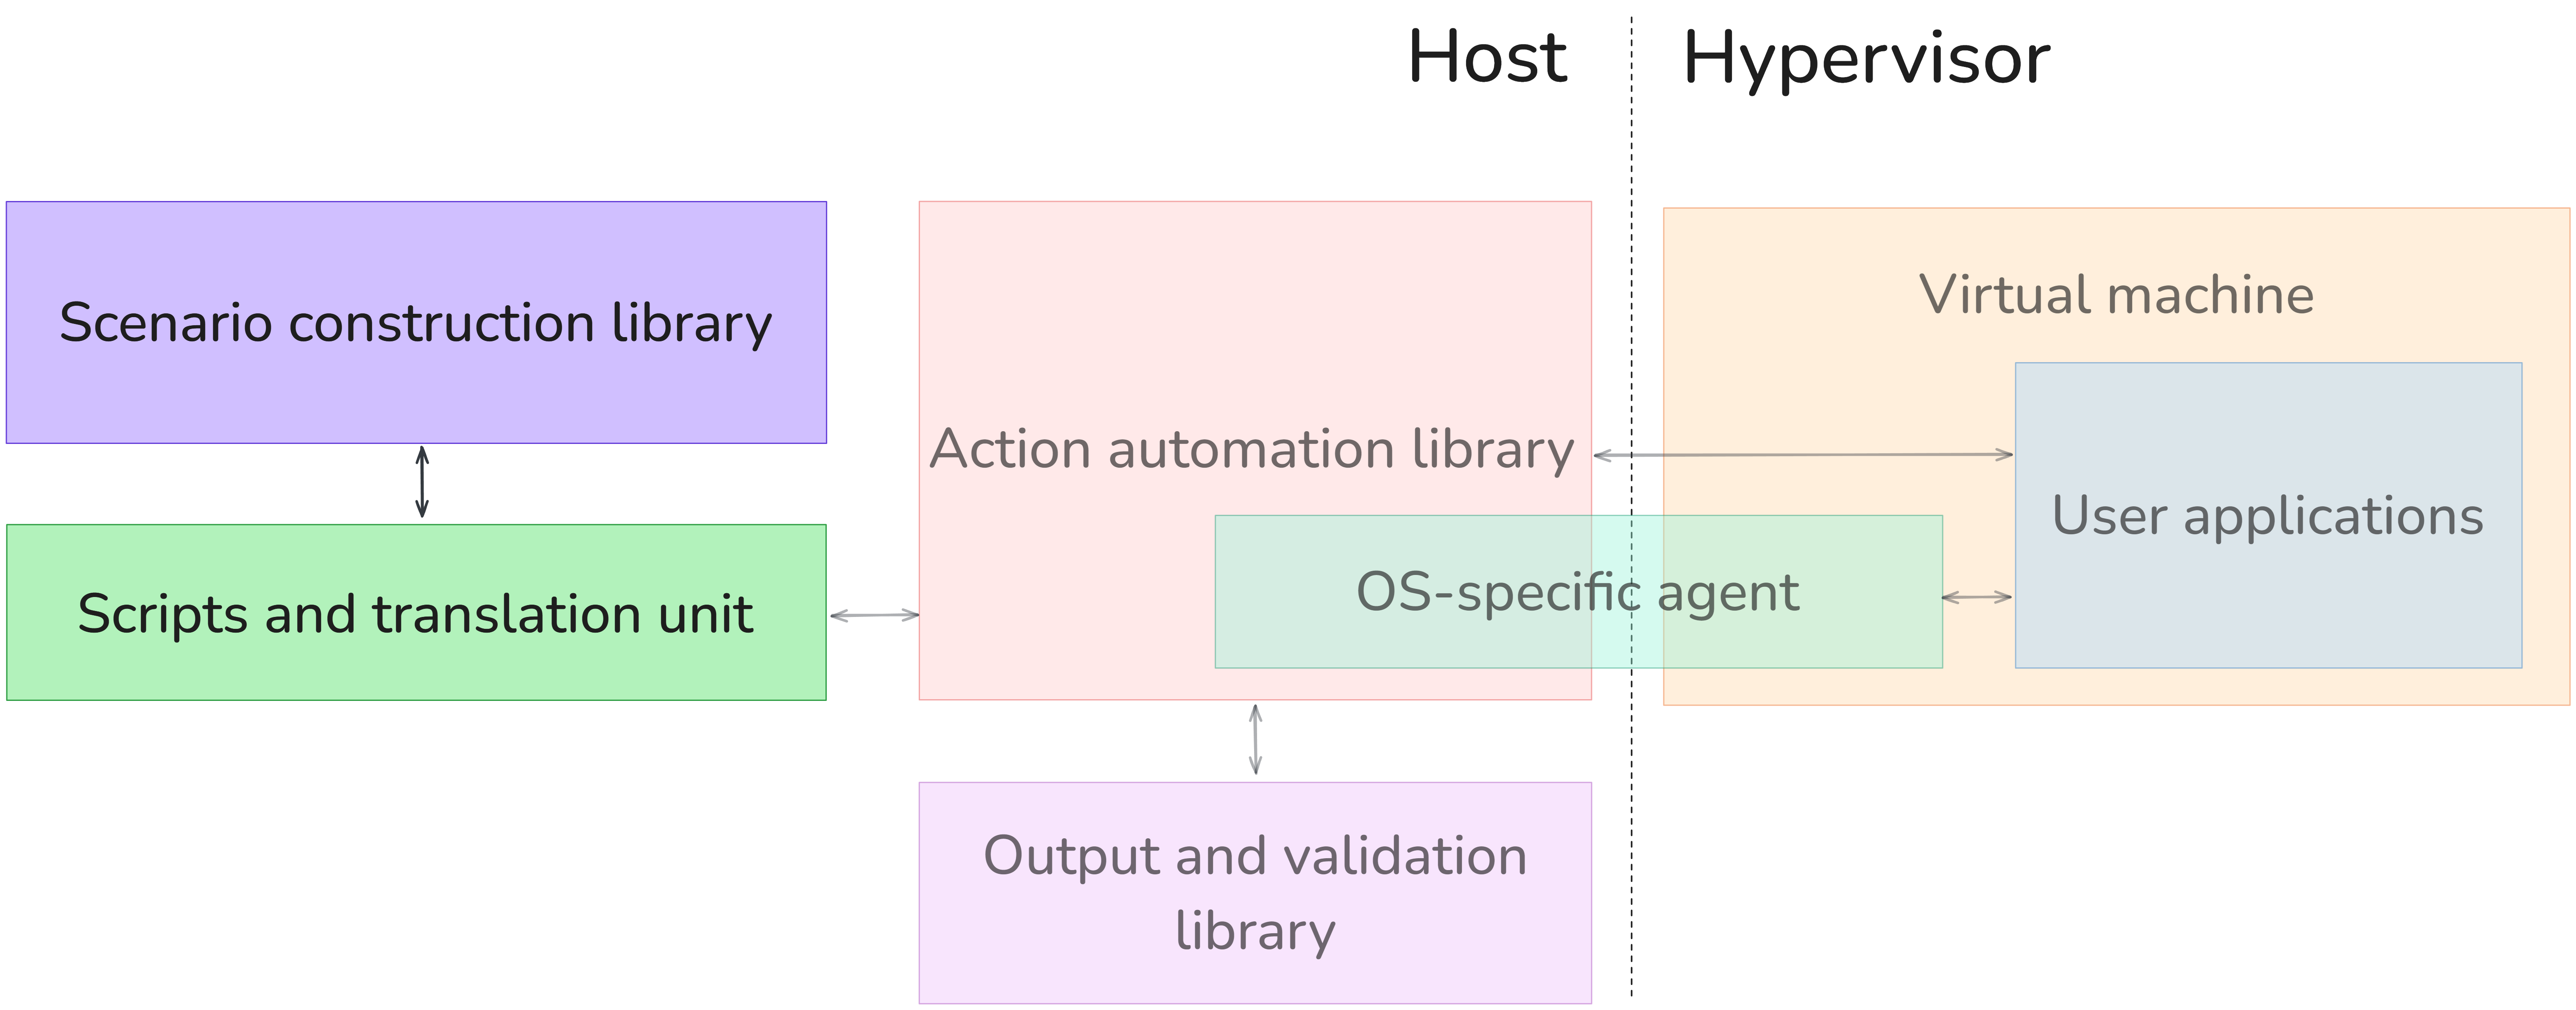
\includegraphics[width=1\linewidth]{scenarios-simple.png}
\caption{Simplified AKF architecture diagram for scenario construction
modules}\label{fig:scenarios-simple}
\end{figure}

At this point, we have provided the functionality for automating
artifact generation in a near-deterministic manner with comprehensive
logging and reporting. However, there is still the challenge of exposing
this functionality in a user-friendly manner. At a high level, there are
two primary ways to define an input to a synthesizer. These formats
describe the process (the \emph{how}) of placing artifacts and
performing actions:

\begin{itemize}
\tightlist
\item
  An \textbf{imperative} format, in which the synthesizer is provided
  instructions in an imperative programming language, and the developer
  must provide the exact instructions for the synthesizer to take
  through some exposed API.
\item
  A \textbf{declarative} format, in which the synthesizer is provided a
  file that describes the desired elements of the result, and it is up
  to the synthesizer to execute the instructions necessary to achieve
  the result.
\end{itemize}

However, the challenge of deciding \emph{what} actions to perform
remains. It is still mainly the responsibility of instructors to provide
background noise and other realistic artifacts to insert into a
scenario. Additionally, although synthesizers make it easier to place
files at desired locations or visit websites, these scenario elements
must be defined and created beforehand. More precisely, these represent
challenges in two specific areas:

\begin{itemize}
\tightlist
\item
  \textbf{Generating standalone artifacts}: Users must include email
  conversations, documents, and other application-specific artifacts to
  be generated as part of a scenario.
\item
  \textbf{Creating the scenario itself}: Users must combine these
  standalone artifacts to generate a cohesive scenario, following a
  theme such as corporate espionage or ransomware attacks.
\end{itemize}

This chapter addresses the challenges of providing APIs for complex
GUI-driven applications and creating background noise. More precisely,
we address two questions -- how do we invoke AKF's automation systems,
and how does AKF assist a user in building a scenario? Here, we explore
AKF's imperative and declarative syntaxes and the viability of using
generative AI to assist in building individual files and complete
scenario descriptions.

\section{Scripting background}\label{scripting-background}

We begin by analyzing how synthesizers accept instructions for execution
-- more precisely, how do users define the sequence of operations that
the synthesizer should take to create the dataset?

For many of the frameworks created in the last decade, users define
scenarios by using a Python library to interact with the framework. The
library is responsible for setting up the virtualized environment and
performing high-level actions on the environment, abstracting away the
underlying calls to the hypervisor from the scenario developer. This
code-based approach represents an \emph{imperative} strategy for
scenario creation, where the user describes how the dataset should be
created by defining the exact order and means to perform synthesizer
actions. It is worth noting that the language used to interact with the
synthesizer's API does not need to match the language used to implement
the synthesizer itself, although this is often the case. For example,
the automation framework Playwright is implemented in TypeScript,
initially exposing a Node.JS API
\cite{MicrosoftPlaywrightpython2025}; today, Playwright provides
APIs in Python, Java, and C\#.

In contrast, custom scenario formats provided by D-FET
\cite{williamCloudbasedDigitalForensics2011}, SFX
\cite{russellForensicImageDescription2012}, and Yannikos et al.
\cite{yannikosDataCorporaDigital2014} follow a different approach.
For these synthesizers, a custom high-level language describes the
desired final state of the dataset. Instead of importing libraries and
writing code, users state the desired elements of the forensic dataset,
allowing the synthesizer to decide how to create the desired dataset --
a \emph{declarative} strategy for scenario creation. The specifics of
state management and execution are delegated to the synthesizer.

Consider the following declarative SFX code taken from Russell et
al.~shown in \autoref{lst:6.1a}
\cite{russellForensicImageDescription2012}:

\begin{lstlisting}[label={lst:6.1a}, caption={Declarative SFX scenario with web browsing \cite{russellForensicImageDescription2012}}, language=XML]
<disk>
    <partition index="p1" hidden="0" size="48M" type="ntfs">
        <base os="windows7x64"/>
        <user username = "Gordon">
             <browserhistory browser="firefox">
                 <url link="bbc.co.uk" time="13:14:00 1 Jan 2013"/>
             </browserhistory>
        </user>
    </partition>
</disk>
\end{lstlisting}

Here, a Windows 7 partition is created as part of a larger disk image.
The partition is loaded in a virtual machine to create a user called
``Gordon,'' who uses Firefox to browse the internet. (This simple web
browsing scenario will be reused throughout this chapter to demonstrate
several code examples.)

The same might be expressed in ForTrace
\cite{gobelForTraceHolisticForensic2022} as shown in
\autoref{lst:6.1b}, excluding additional code required for ground truth
and disk image generation:

\begin{lstlisting}[label={lst:6.1b}, caption={Imperative ForTrace scenario with web browsing \cite{gobelForTraceHolisticForensic2022}}, language=Python]
from fortrace.core.vmm import Vmm
from fortrace.utility.logger_helper import create_logger
from fortrace.core.vmm import GuestListener

if __name__ == "__main__":
    logger = create_logger('fortraceManager', logging.DEBUG)
    macsInUse = []
    guests = []
    
    guestListener = GuestListener(guests, logger)
    virtual_machine_monitor1 = Vmm(macsInUse, guests, logger)
    # boottime expressed as "%Y-%m-%d %H:%M:%S"
    guest = virtual_machine_monitor1.create_guest(guest_name="w-guest01", platform="windows", boottime="2013-01-01 13:14:00")

    browser_obj = guest.application("webBrowserFirefox", {'webBrowser': "firefox"})
    browser_obj.open(url="bbc.co.uk")
    while browser_obj.is_busy:
        time.sleep(2)
    browser_obj.close()
\end{lstlisting}

Although these two code blocks have the same expressive power (that is,
they achieve the same overall outcomes), there is a clear difference in
the complexity and length between them. It is significantly easier to
read and write the declarative XML in the first code block, as it
abstracts away the need to instantiate various synthesizer objects and
call specific methods. By extension, this also allows for a common
declarative syntax to be used across multiple synthesizers since
low-level synthesizer details do not need to be exposed as part of the
declarative syntax.

The primary benefit of an imperative approach to generation is its
flexibility; on a Python-based synthesizer, one can simply import
another library to extend the functionality of the base scenario
definition. This flexibility naturally comes at the expense of a greater
learning curve. Although many digital forensic specialists are likely to
have programming experience, it is far easier to learn a restricted
declarative specification (like XML) than an entire programming
language, which may entail additional setup (such as installing an IDE,
dependencies, and so on).

When accessibility is preferred over functionality, declarative syntaxes
can be more valuable than imperative syntaxes. Some scenario developers,
such as classroom instructors, may not need the low-level control
provided by an imperative syntax or a complete programming language such
as Python. It also takes time to learn about the functionality exposed
by the synthesizer's library, not to mention learning the programming
language itself. These are the primary motivators behind supporting
well-defined declarative syntaxes.

Of course, low-level control is still important, especially when
external libraries must be used to implement functionality not
inherently exposed by a synthesizer. For this reason, some synthesizers
support both declarative and imperative scripts to generate scenarios.
For example, the Python-based hystck and ForTrace frameworks
\cite{gobelNovelApproachGenerating2020,gobelForTraceHolisticForensic2022}
allow users to write YAML scripts to execute actions. Support for both
formats can be implemented through various means, such as
declarative-to-imperative translators. (While not explored in this
thesis, it is also worth noting the GUI-based interfaces provided by
Yannikos et al. \cite{yannikosDataCorporaDigital2014} and ForGe
\cite{vistiAutomaticCreationComputer2015} for building scenarios.)

AKF supports an imperative syntax (through its Python API) and a custom
declarative syntax. Unlike prior synthesizers, AKF's declarative syntax
supports both execution and declarative-to-imperative translation,
allowing users to quickly create and modify imperative scripts from
high-level declarative descriptions.

\section{Setup and basic usage}\label{setup-and-basic-usage}

Like many of its predecessors, AKF implements its functionality and
exposes its API in the same language, Python 3. There are numerous
advantages to a Python-based API; besides the relatively low difficulty
of setting up and using Python, its rich ecosystem allows scenarios to
be extended through other libraries from the Python ecosystem. For
example, if a user wanted to conditionally execute certain parts of a
scenario by testing if a particular remote service is currently online,
a user could use the Requests library \cite{Requests31Documentation}
to issue an HTTP request out-of-band before performing the same action
in a virtualized environment.

Users must install two foundational technologies for AKF to operate --
Python 3.11 (or later) and a supported hypervisor. AKF currently only
supports VirtualBox as its hypervisor, though QEMU/libvirt has also been
used in prior synthesizers. AKF uses
\passthrough{\lstinline!pyproject.toml!} to define Python library
dependencies, which can be installed into a virtual environment using a
package manager such as \passthrough{\lstinline!pip!} or
\passthrough{\lstinline!uv!}.

At this point, a virtual machine must be prepared for use with AKF. As
with prior synthesizers, it is possible to manually configure a machine
by downloading a supported operating system and creating a new virtual
machine from scratch. The manual process, which is similar to that of
other synthesizers, is as follows:

\begin{itemize}
\tightlist
\item
  Download an ISO or pre-prepared virtual machine from a distributor
  with the desired operating system.
\item
  If necessary, install the operating system on a new virtual machine.
\item
  Configure the virtual machine with the desired host resources,
  including two network interfaces -- one connected to the NAT adapter
  for general internet usage and one connected to the host-only adapter
  for agent communications.
\item
  Create an administrative user with known credentials. Configure the
  operating system as desired to reduce friction with the synthesizer
  (such as disabling UAC prompts, enabling auto-logon, and so on.)
\item
  Build and copy the OS-specific AKF agent to the virtual machine,
  configuring it as a startup application. Add firewall rules to ensure
  that the host and agent are able to communicate.
\end{itemize}

After this process, the virtual machine can be cloned and reused in
multiple AKF scenarios. Although relatively straightforward, this
process is still time-consuming, especially when adapted to new
operating systems. While a prepared AKF virtual machine can
theoretically be distributed (in a virtual appliance format such as
OVF), this can run into legal issues if the software on the underlying
operating system is copyrighted.

As a result, AKF uses modern infrastructure-as-code solutions to vastly
simplify the setup of new virtual machines. Vagrant, developed by
HashiCorp, is a tool for rapidly building development environments
\cite{HashicorpVagrant2025}. It allows users to define and build
virtual machines on several virtualization platforms, including
VirtualBox and VMWare. Virtual machines are built by configuring a base
image according to a Vagrantfile, which describes hypervisor-specific
configuration options and instructions to configure the machine. The
Vagrantfile can be distributed to users, allowing them to build the same
virtual machine without distributing virtual drives. (A similar approach
of distributing the ``differences'' of base images is used to reduce the
size of distributed forensic datasets by EviPlant
\cite{scanlonEviPlantEfficientDigital2017}, as described in
\autoref{distribution}.)

The AKF Windows agent includes a Vagrantfile for creating a new Windows
11 virtual machine with the agent installed and configured, which can
easily be adapted for other platforms and hypervisors. The
Vagrantfile(s) used to generate a dataset should be included with the
dataset itself to maximize reproducibility, as described in \autoref{distribution-and-community-reproducibility}. A robust ecosystem of Vagrant boxes for varying Linux
distributions and Windows versions exists, many of which can be pulled
from the Vagrant public registry
\cite{hashicorpHashiCorpCloudPlatform}. When combined with the
flexibility of Vagrant over multiple virtualization platforms, this can
significantly improve the reproducibility and usability of AKF across
many platforms. It should also be noted that Vagrant can configure and
build larger environments with multiple machines. For organizations that
can express corporate environments as Vagrantfiles, AKF could perform
artifact generation at scale, allowing for incident response scenarios
reflecting real-world networks and events.

Following setup, developers can build scenarios using the AKF core
libraries (\passthrough{\lstinline!akflib!}) and the API of the
platform-specific agent installed onto the virtual machine. This
reflects typical imperative usage, in which environment setup, artifact
generation, and output generation are handled explicitly through a
script executed through the Python interpreter.

A simple AKF script achieving the same outcomes as the ForTrace and SFX
scripts above is shown in \autoref{lst:6.2a}:

\begin{lstlisting}[label={lst:6.2a}, caption={Example of an imperative AKF scenario}, language=Python]
from akf_windows.api.chromium import ChromiumServiceAPI
from akflib.core.hypervisor.vbox import VBoxExportFormatEnum
from akflib.core.hypervisor.vbox import VBoxHypervisor
from pathlib import Path

# Instantiate a hypervisor object tied to a specific virtual machine
vbox_obj = VBoxHypervisor("akf-windows-1")

# Start the virtual machine
vbox_obj.start_vm(wait_for_guest_additions=True)

# Visit a single website
with ChromiumServiceAPI.auto_connect(vbox_obj.get_maintenance_ip()) as chromium_service:
    chromium_service.kill_edge()
    chromium_service.set_browser("msedge")
    page = chromium_service.browser.new_page()
    page.goto("bbc.co.uk")  

# Stop the virtual machine
vbox_obj.stop_vm(force=False)

# Export the virtual machine to a disk image
vbox_obj.create_disk_image(
    Path("C:/Users/kisun/Desktop/akf-windows_1.raw"),
    VBoxExportFormatEnum.RAW
)
\end{lstlisting}

Here, we create a new \passthrough{\lstinline!VBoxHypervisor!} instance
that will allow us to start and interact with a VirtualBox machine
called \passthrough{\lstinline!akf-windows-1!} (created previously with
Vagrant as described above). To initialize the Chromium subservice, we
query VirtualBox for the IP address of the host-only adapter, then use
the \passthrough{\lstinline!auto\_connect!} convenience method to
automatically perform the required RPyC setup and return an instance of
\passthrough{\lstinline!ChromiumServiceAPI!}. This instantiated API
allows us to interact with Microsoft Edge on the virtual machine over
RPyC (which is abstracted away from the user); as part of the context
manager, the RPyC connection is automatically closed at the end of the
\passthrough{\lstinline!with!} block. Finally, we create a raw disk
image and save it to the desktop.

With this in mind, how do we expose this same functionality through a
declarative syntax?

\section{Declarative usage}\label{declarative-usage}

As described previously, declarative inputs are well-structured files
with a fixed set of available actions -- effectively forming an API --
where each entry in the file specifies an action or artifact to be
generated as part of a dataset. Individual entries may contain
additional configuration data that modifies how that specific action or
artifact is generated. An \emph{interpreter} is responsible for parsing
and acting on the entries in the declarative file.

Interpreters can act on declarative formats in one of two ways. The
first is \emph{execution}, in which the elements of the declarative
script are directly interpreted to generate imperative API calls. This
is characteristic of synthesizers that only support declarative script
inputs, exposing no low-level APIs. Execution takes advantage of the
high-level nature of declarative scripts; a declarative script can
remain the same even if the libraries that execute it change, so long as
the interpreter is updated accordingly. The second is
\emph{translation}, in which the declarative script is used to generate
an equivalent imperative script adhering to a particular synthesizer's
API. This allows the declarative script to be used as a ``base'' for
creating imperative scripts, such that an experienced scenario developer
can modify the generated imperative script as needed. Imperative scripts
can be regenerated from the same declarative script to reflect updates
in library usage so long as the interpreter is updated accordingly,
inheriting the evergreen nature of declarative scripts.

It is important to note that a declarative syntax, which may be more
``rigid'' in structure, does not preclude the use of non-determinism or
randomness. One notable example of this is the discrete-time Markov
chains used by Yannikos et al.~to express scenarios in a probabilistic
manner, with each state of the Markov chain representing a particular
action taken by the synthesizer (such as sending an email or deleting a
file) \cite{yannikosDataCorporaDigital2014}. These chains are
evaluated at runtime to generate multiple unique datasets from a single
description.

The challenges of defining a suitable declarative syntax for a
particular synthesizer are not unlike the challenges faced in general
programming language design. There are several key factors to the
success of imperative programming languages that extend to declarative
syntaxes, some of which are derived from Finkel and described as follows
\cite{finkel1996advanced}:

\begin{itemize}
\tightlist
\item
  The language should be \textbf{simple}, using as few basic concepts as
  possible. This makes code easier to read and write, an important
  aspect for users with limited programming experience.
\item
  The language should be \textbf{modular}, such that the role and
  interfaces of individual program units are clear.
\item
  The language should be \textbf{predictable}, such that users can apply
  their existing knowledge of a synthesizer to quickly implement or add
  new features to a scenario.
\item
  The language should \textbf{abstract} as much as possible away from
  the user, such that the minimum information needed to fulfill artifact
  generation is exposed to the user.
\end{itemize}

The most important factor, however, is an awareness of the
\textbf{purpose} of the declarative syntax. The purpose of a synthesizer
is to make it easier to generate forensic artifacts and datasets. The
declarative language should reflect this, focusing on making actions and
artifacts as easy to declare and customize as possible. (These five
factors are particularly important in allowing LLMs to reliably generate
declarative scenarios, as described in \autoref{using-llms-for-high-level-scenarios}.)

In designing the AKF declarative syntax, the declarative syntaxes of
prior synthesizers and unrelated technologies were evaluated. An
analysis of some of these syntaxes, with examples, is described briefly
in \autoref{historical-declarative-syntaxes}.
However, the two syntaxes that contributed most to the AKF declarative
syntax were those of ForTrace and Ansible, described in the following
section.

\subsection{Existing declarative
syntaxes}\label{existing-declarative-syntaxes}

ForTrace \cite{gobelForTraceHolisticForensic2022} uses YAML to
express scenarios in a declarative manner. ForTrace significantly
influenced both the AKF declarative syntax itself and the implementation
of the declarative interpreter, primarily because it was the sole
open-source synthesizer with both imperative and declarative support.
\autoref{lst:6.3.1a} demonstrates a simple example of a ForTrace
declarative scenario:

\begin{lstlisting}[label={lst:6.3.1a}, caption={Declarative ForTrace scenario with web browsing \cite{gobelForTraceHolisticForensic2022}}, ]
name: haystack-example
description: A example action suite to generate a haystack (traffic)
author: MPSE Group
seed: 1234
collections:
  c-http-0:
    type: http
    urls: ./generator/friendly_urls.txt
settings:
  host_nfs_path:
  guest_nfs_path:
applications:
hay:
  h-http-0:
    application: http
    amount: 3
    collection: c-http-0
needles:
  n-http-0:
    application: http
    url: dasec.h-da.de
    amount: 1
dumps:
  d-dump-0:
    dump-type: mem
    dump-path: /home/fortrace/gendump.file
\end{lstlisting}

At a high level, ForTrace scenarios contain five distinct elements:

\begin{itemize}
\tightlist
\item
  Metadata about the scenario, such as the scenario's name, description,
  and author.
\item
  ``Collections'' of data that can be reused throughout the scenario in
  supported application types, such as a newline-separated list of URLs.
\item
  Configuration options that may be applied to all actions of a
  particular action type or the entire scenario.
\item
  The actual artifacts to create as part of the
  \passthrough{\lstinline!hay!} and \passthrough{\lstinline!needles!}
  sections, where \passthrough{\lstinline!hay!} includes artifacts that
  should be considered background noise, and
  \passthrough{\lstinline!needles!} includes artifacts that should be
  considered significant. Each artifact contains a unique ID, an
  application type (the \passthrough{\lstinline!application!} key), and
  arguments specific to the application responsible for generating the
  artifact, such as the URLs for web browsing.
\item
  Any core outputs that should be created as part of the scenario.
\end{itemize}

This file is passed into a ``generator,'' which parses the contents of
the YAML file to prepare various internal data structures, initialize
the virtual machine, and then execute the actions specified in the
\passthrough{\lstinline!hay!} and \passthrough{\lstinline!needles!}
sections in a random order according to the
\passthrough{\lstinline!seed!} key. Depending on the value of the
\passthrough{\lstinline!application!} key, the data for that action is
passed to an application-specific handler that interacts with the
running virtual machine using existing ForTrace libraries. Once all the
actions have been executed, the generator creates any requested outputs
(such as volatile memory dumps) and shuts down the virtual machine.

This analysis provided insight into the design decisions and
functionality required to execute actions from the high-level
descriptions of a scenario. In particular, it demonstrates the need for
actions or artifacts to be defined consistently and flexibly so that
program state and other data can be passed to application-specific
libraries as needed. It also demonstrates the need for various levels of
configuration, including scenario-wide configuration,
application-specific configuration, and action/artifact-specific
configuration. ForTrace implements these features in a somewhat awkward
manner; in fact, nearly all declarative language support is contained in
a single file, with a hardcoded ``router'' handling each unique
\passthrough{\lstinline!application!} type. This makes it difficult to
add support for new applications without significant effort,
particularly because the generator must be aware of every possible
action/artifact type ahead of time.

With these priorities and issues from ForTrace identified, are there
ideas from other technologies that can be used to address them? That is,
are there other technologies designed to execute a large set of complex
actions using a simple but flexible and configurable syntax, and how
does it work? Ansible, the second major inspiration for the AKF
declarative syntax, precisely addresses these questions.

Ansible \cite{AnsibleAnsible2025} is an open-source automation
framework often used to remotely configure Windows and Linux machines at
scale, allowing organizations to manage many machines at once without
installing orchestration software on these machines in advance. To
achieve this, users write \emph{playbooks}, which are simple YAML files
that contain one or more \emph{plays}. Each play is simply a set of
\emph{tasks} run on multiple machines simultaneously, and each task
depends on a \emph{module} designed to achieve a single, specific
outcome.

An example of an Ansible playbook can be seen in \autoref{lst:6.3.1b},
which contains a single play to configure an Apache webserver.

\begin{lstlisting}[label={lst:6.3.1b}, caption={Minimal Ansible playbook for updating an Apache server \cite{ansibleprojectcontributorsAnsiblePlaybooks}}, ]

- name: Update web servers
  hosts: webservers
  remote_user: root
  tasks:
  - name: Ensure apache is at the latest version
    ansible.builtin.yum:
      name: httpd
      state: latest
  - name: Write the apache config file
    ansible.builtin.template:
      src: /srv/httpd.j2
      dest: /etc/httpd.conf
\end{lstlisting}

This play uses the \passthrough{\lstinline!yum!} package manager to
install Apache before copying a local configuration file to the remote
host. \passthrough{\lstinline!ansible.builtin.yum!} and
\passthrough{\lstinline!ansible.builtin.template!} are both modules,
which accept parameters passed as a YAML dictionary. These modules are
part of the \passthrough{\lstinline!ansible.builtin!} collection
included with all default Ansible installations.

Although Ansible contains many features that contribute to its
flexibility, the two important concepts relevant to AKF are \emph{roles}
and \emph{modules}. Roles are a collection of Ansible resources that
achieve some ``larger'' reproducible goal, typically by leveraging
tasks, variables, configuration options, and files included as part of
the role. Roles can include \emph{modules}, which are standalone
imperative scripts (typically in Python) that accept arguments, execute
code based on those arguments, and return data using well-structured
interfaces. As shown above, these modules can be called and executed
from playbooks; they can also be executed independently on the command
line.

These concepts are highly relevant to synthesizers, which must support
application-specific actions and group these actions together in a
flexible, well-defined manner. As described in \autoref{the-akf-agent}, each RPyC subservice of an AKF agent
exposes a group of application-specific automation methods. The
functionality of each of these groups must be re-exposed in a
declarative manner, which can be achieved by adapting the concept of
Ansible roles and modules to AKF.

Together, the ForTrace and Ansible syntaxes provide three concepts that
are reflected in the AKF syntax, described further in the following
section:

\begin{itemize}
\tightlist
\item
  The overall structure and contents of the declarative YAML file.
\item
  An action syntax that allows us to declare individual actions,
  referring to those actions by name, and pass arguments directly to
  that action for \emph{translation} or \emph{execution}.
\item
  A modular architecture that allows us to define the supported
  arguments of each action and expose them to the declarative
  interpreter while also being decoupled from the standard imperative
  library as much as possible.
\end{itemize}

\subsection{The AKF declarative
syntax}\label{the-akf-declarative-syntax}

The AKF declarative syntax is very similar to the Ansible playbook
syntax. Declarative scripts are comprised of metadata, global
configuration, libraries to import, and individual tasks to execute as
part of the scenario. Each task refers to a single \emph{module} by name
using a qualified Python import path, accepting a dictionary of
arguments in addition to global configuration overrides.

Like Ansible, individual modules are implemented as well-defined
subclasses of \passthrough{\lstinline!AKFModule!}, an abstract base
class that serves as the root of all AKF declarative modules. Each
module must define Pydantic models that specify the arguments accepted
by the module. The arguments declared in the YAML file are then passed
to these module-specific Pydantic models for validation, after which the
\passthrough{\lstinline!AKFModule!} must perform one of two tasks:

\begin{itemize}
\tightlist
\item
  \textbf{Execution}: When instructed to perform actions directly from
  the declarative script, the \passthrough{\lstinline!AKFModule!} should
  import AKF core libraries and agent APIs to perform the required
  actions.
\item
  \textbf{Translation}: When instructed to translate the declarative
  script, the \passthrough{\lstinline!AKFModule!} should generate the
  equivalent code that \emph{would} perform the required actions if
  executed through a standard Python interpreter with the necessary
  libraries installed.
\end{itemize}

The ability of AKF to both execute and translate declarative scripts
provides significant flexibility to scenario developers. To the best of
our knowledge, prior synthesizers have only supported direct execution
from declarative scripts, which limits the opportunities to use
declarative scripts as a ``starting point'' for writing more complex
imperative scripts. (In fact, the code in \autoref{lst:6.2a} was
primarily derived from the auto-generated code shown in
\autoref{lst:6.3.2a}.)

An example of a minimal AKF scenario, carrying out the same actions as
the SFX, ForTrace, and imperative AKF script above, can be seen in
\autoref{lst:6.3.2a}:

\begin{lstlisting}[label={lst:6.3.2a}, caption={Example of a declarative AKF scenario}, ]
name: Minimal scenario
description: Browses to the BBC website and exports a disk image.
author: Lloyd Gonzales
seed: "0"
libraries:
  - akflib.modules
  - akf_windows.modules
actions:
  - name: Instantiate a hypervisor object tied to a specific virtual machine
    module: vbox_start
    args:
      machine_name: "akf-windows-1"
  - name: Start the virtual machine
    module: vbox_start_machine

  # Visit a website using Microsoft Edge. A temporary instance of the Chromium
  # subservice API is created for the lifetime of this module.
  - name: Visit a single website
    module: chromium_visit_urls
    args:
      browser: "msedge"
      urls: 
       - "bbc.co.uk"

  # Stop the virtual machine and export the virtual machine to a disk image.
  - name: Stop the virtual machine
    module: vbox_stop_machine
    args:
      force: false
  - name: Export the virtual machine to a disk image
    module: vbox_create_disk_image
    args:
      output_path: "C:/Users/user/Desktop/akf-windows_1.raw"
      image_format: "raw"
\end{lstlisting}

The \passthrough{\lstinline!akf-translate!} interpreter, which is added
to PATH when installing \passthrough{\lstinline!akflib!}, handles both
execution and translation from a declarative script. It uses the same
underlying library calls as the imperative code in \autoref{lst:6.2a}.
To use this declarative script with
\passthrough{\lstinline!akf-translate!}, one of the following commands
in \autoref{lst:6.3.2b} can be used:

\begin{lstlisting}[label={lst:6.3.2b}, caption={Sample usage of the akf-translate utility}, language=sh]
# Translate this scenario to a valid Python script and save it to disk
akf-translate scenarios/thesis.yaml --translate --output-file scenarios/thesis.py

# Execute this scenario directly
akf-translate scenarios/thesis.yaml --execute
\end{lstlisting}

AKF declarative scripts, which are simply large YAML dictionaries,
contain three distinct elements. The first is a set of high-level
metadata keys associated with the scenario. The second is a set of
scenario-wide configurations; in particular, it lists the libraries
containing the necessary modules to execute or translate this imperative
script. Finally, scripts list a sequence of actions, typically a
\passthrough{\lstinline!module!} specified by name and a dictionary of
\passthrough{\lstinline!args!}.

The execution flow of \passthrough{\lstinline!akf-translate!} itself is
straightforward. Given a path to a YAML script, the interpreter will
load the necessary libraries and configuration keys defined in the file
and instantiate resources accordingly. This may include setting aliases
for module names, verifying that all required modules are available,
setting the \passthrough{\lstinline!random!} seed, and so on. Then, the
interpreter runs each module under the \passthrough{\lstinline!actions!}
key with the provided arguments and configuration in order, continuing
until all actions have been processed.

Modules can read and modify a global state dictionary that allows
otherwise independent modules to cooperate. For example, suppose that a
module creates a new context manager in a \passthrough{\lstinline!with!}
block, causing the indentation level of the translated code to increase.
Successive modules can read the state dictionary to retrieve context
variables and correctly indent generated code. Additionally, this allows
for ``outputs,'' such as CASE bundles, to be passed and gradually
constructed across modules. This design allows for context-aware code
generation and action execution.

Modules are located and executed using Python's dynamic import system.
These modules can be located in any library so long as they can be found
through Python's import system. For example, both
\passthrough{\lstinline!akflib!} and the AKF Windows agent contain their
own declarative module libraries, leveraging functionality specific to
each code repository. All modules in the script are located and
``cached'' at the start of script execution, which allows for
verification and runtime efficiency.

This design allows declarative modules to be written independently of
the libraries they depend on, reducing the ``impact'' of supporting
declarative features on the core imperative libraries. In fact, this
independence allows for the AKF module system to be used in
general-purpose scripting, similar to Ansible; it is not tightly bound
to the creation of forensic scenarios and artifacts. That said, the
existing declarative modules of AKF expose nearly all existing
functionality provided by \passthrough{\lstinline!akflib!}, including
PDF report generation, virtual machine interaction, and more.

The list of declarative modules available through
\passthrough{\lstinline!akflib!} and the Windows agent is described in
\autoref{tbl:akf-declarative-modules} below. Note that these modules are
referred to by their alias, not their fully-qualified module paths.


{
\small % 10pt font
\setstretch{1} % Single spacing
\begin{longtable}[]{@{}
  >{\raggedright\arraybackslash}p{(\linewidth - 2\tabcolsep) * \real{0.3}}
  >{\raggedright\arraybackslash}p{(\linewidth - 2\tabcolsep) * \real{0.7}}
@{}}
\caption{Available AKF declarative modules}\label{tbl:akf-declarative-modules} \\
\toprule\noalign{}
\begin{minipage}[b]{\linewidth}\raggedright
Name
\end{minipage} & \begin{minipage}[b]{\linewidth}\raggedright
Description
\end{minipage} \\
\midrule\noalign{}
\endhead
\bottomrule\noalign{}
\endlastfoot
\passthrough{\lstinline!create\_akf\_bundle!} & Creates a new CASE
bundle for use throughout the declarative scenario. \\
\passthrough{\lstinline!write\_akf\_bundle!} & Write the contents of the
currently active CASE bundle to disk as a JSON-LD file. \\
\passthrough{\lstinline!render\_akf\_bundle!} & Pass the currently
active CASE bundle through a set of provided renderers and construct a
valid PDF using Pandoc. \\
\passthrough{\lstinline!vbox\_start!} & Create a new VirtualBox instance
bound to a specific virtual machine by name. \\
\passthrough{\lstinline!vbox\_start\_machine!} & Power on the currently
active virtual machine. \\
\passthrough{\lstinline!vbox\_stop\_machine!} & Power off the currently
active virtual machine. \\
\passthrough{\lstinline!vbox\_create\_disk\_image!} & Export a disk
image of the current virtual machine. \\
\passthrough{\lstinline!artifact\_service\_start!} & Remotely start and
connect to the subservice responsible for collecting Windows
artifacts. \\
\passthrough{\lstinline!artifact\_service\_stop!} & Disconnect from the
subservice responsible for collecting Windows artifacts. \\
\passthrough{\lstinline!prefetch!} & Analyze all prefetch files on disk
and construct their corresponding CASE objects. \\
\passthrough{\lstinline!chromium\_service\_start!} & Remotely start and
connect to the subservice responsible for interacting with Chromium
browsers. \\
\passthrough{\lstinline!chromium\_service\_stop!} & Disconnect from the
subservice responsible for interacting with Chromium browsers. \\
\passthrough{\lstinline!chromium\_visit\_urls!} & Visit one or more URLs
using a specified web browser. \\
\passthrough{\lstinline!chromium\_history!} & Collect browsing history
from a specified web browser and construct their corresponding CASE
objects. \\
\end{longtable}
}


Although these declarative modules (and the imperative library) provide
users with significant flexibility in \emph{using} AKF, there remains
the challenge of building artifacts and scenarios to use with AKF. The
remainder of this chapter addresses this challenge.

\section{Using generative AI for individual
artifacts}\label{using-generative-ai-for-individual-artifacts}

\subsection{Challenges of standalone
artifacts}\label{challenges-of-standalone-artifacts}

Users of synthesizers must still perform a significant amount of work
when generating individual artifacts. More precisely -- although AKF and
other synthesizers can streamline the process of placing and generating
artifacts, users must still provide some of the artifacts themselves.
For example:

\begin{itemize}
\tightlist
\item
  If a user wants to place 100 photos on the drive to simulate real
  usage, the user needs to create and provide 100 realistic images.
\item
  If a user wants to simulate an email or other online conversation, the
  user needs to provide the entirety of the conversation to simulate.
  Such conversations would need to be consistent with the ``theme'' of a
  scenario.
\item
  If a user wants to generate ``proprietary'' documents to emulate some
  form of corporate sabotage, the user would need to create and provide
  a variety of Microsoft Office, PDF, or other files in these formats.
\end{itemize}

This is particularly relevant when adding background noise intended to
emulate benign activity. Such datasets are valuable training material in
forensic courses that encapsulate a long period of study, allowing
students to apply many different techniques learned throughout a
curriculum to analyze a realistic scenario.

Indeed, the artifacts in the bulleted list above are all elements of the
NIST CFReDS Data Leakage Case
\cite{nationalinstituteofstandardsandtechnologyCFReDSDataLeakage},
which contains web browsing history, images, documents, and other media
relevant to the theft of proprietary information related to a product in
development. However, many of these documents are not specific to the
scenario; in particular, the ``technical documents'' present in the
scenario are actually files from the general-purpose Govdocs corpora
\cite{garfinkelBringingScienceDigital2009}, with a cover page
denoting their intended role in the scenario. For example, one
PowerPoint file is portrayed as a presentation of the detailed design of
the product, but its actual contents are that of a Yale University
presentation on brain physiology.

The use of ``irrelevant'' files to portray ``relevant'' files can be
acceptable when the actual content of the artifact is not important in
analyzing the scenario as a whole. This practice significantly reduces
the time spent creating individual artifacts, both those directly
related to the focus of the scenario and those that are intended to be
background noise. However, this technique still detracts from the
realism of the scenario and may not be sufficient to cover all use
cases. One notable example in the Data Leakage Case is the lack of
emails on the device; the sole email conversation is strictly related to
the scenario. A real-world suspect would almost certainly have many
other email conversations consistent with their background, such as
employer-related emails or marketing emails from websites the user has
visited.

Recent advancements in AI models have made it significantly easier to
generate text, images, and other media from high-level descriptions.
Generative AI can quickly populate forensic datasets with realistic
conversations and images consistent with an arbitrary scenario, such as
the scenario presented by the Data Leakage Case. For example, a large
language model (LLM) could be prompted to generate text describing a
fictional piece of machinery in both technical and conversational
styles. The text could then be combined with images generated by another
model to create documents and emails. This provides a pipeline through
which thematically consistent artifacts can be generated and placed onto
a forensic dataset. The same process can be performed for artifacts that
are simply background noise; generating hundreds of ``irrelevant''
emails would be impractical for a human but trivial for an LLM.

This idea can be extended further by training models on specific
datasets; for example, if an instructor wished to create a fictional
scenario in which a user frequently interacts with users of a particular
online community, a large language model could be trained on (or
otherwise provided) existing conversations to provide a degree of
realism to the scenario. However, this faces the challenges of
ownership, privacy, and legality behind works derived from publicly
available information that was not published with the expectation of its
usage in an AI model -- issues very similar to those described in
\autoref{motivation-for-synthetic-datasets}.

It is important to note that the inclusion of generative AI into
synthesizers does not necessarily require deep integration with the
framework itself. Many existing synthesizers could be extended to use
documents, images, or other data sourced from generative AI instead of
user-defined files without significantly changing the synthesizer's
architecture. Directly integrating AI-driven actions into synthesizers
is addressed further in \autoref{open-ended-automation-with-ai}.

\subsection{Building sample standalone
artifacts}\label{building-sample-standalone-artifacts}

This section explores the use of DeepSeek-R1
\cite{deepseek-aiDeepSeekR1IncentivizingReasoning2025} and SDXL 1.0
\cite{podellSDXLImprovingLatent2023} in constructing various
scenario artifacts. In particular, we focus on building artifacts
similar in quality and theme to those found in the NIST CFReDS Data
Leakage Case. Note that the approach detailed below can be generalized
to other models, not just DeepSeek-R1 and SDXL.

As described previously, the Data Leakage Case contained files presented
as technical documentation but had content that was irrelevant to the
scenario itself. Our goal is to create comparable documents containing
text and images consistent with a theme provided to the models
responsible for generating this content. We introduce a three-step
process for generating multimedia artifacts:

\begin{itemize}
\tightlist
\item
  \textbf{Text and prompt generation}: A prompt is provided to
  DeepSeek-R1 to create Markdown document(s) consistent with the
  scenario. Using a special syntax, the model is also instructed to
  insert suitable image generation prompts throughout the document. The
  syntax allows the model to configure image parameters, such as the
  size of the image.
\item
  \textbf{Image generation}: The prompts are extracted from the Markdown
  document and passed to SDXL 1.0. The resulting images are saved to a
  temporary folder, and the special syntax is replaced with the standard
  Markdown syntax for embedding images at a known path.
\item
  \textbf{Rendering}: The resulting Markdown document is passed to a
  tool such as Pandoc to generate the final artifact, similar to the
  approach in \autoref{human-readable-reporting}. Pandoc supports various formats, including PDFs, Microsoft
  Word, and Microsoft PowerPoint. Other tools could be used to convert
  Markdown to other formats.
\end{itemize}

The document snippet shown in \autoref{fig:artifact-document-example}
was produced by following the steps above on locally hosted instances of
DeepSeek-R1 and SDXL 1.0, using Ollama \cite{OllamaOllama2025} and
ComfyUI \cite{comfyanonymousComfyanonymousComfyUI2025} as
interfaces. An instance of \passthrough{\lstinline!deepseek-r1:32b!} was
directed to create a document describing the technical details of a
fictional semiconductor manufacturing product under various constraints.

\begin{figure}[htbp]
\centering
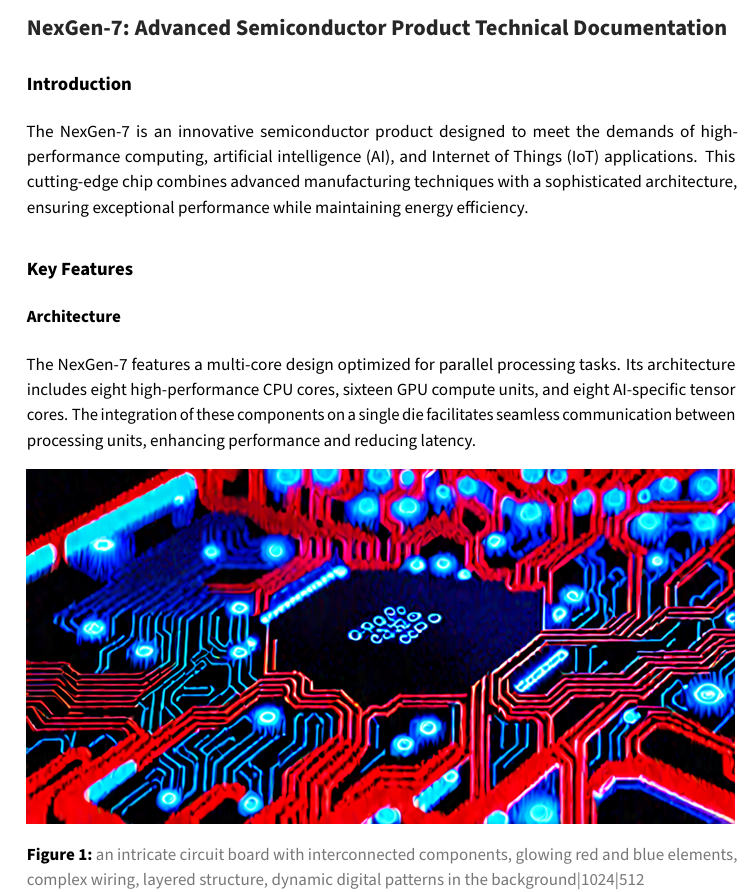
\includegraphics[width=1\linewidth]{pdf-example.png}
\caption{Sample of an AI-generated PDF artifact to be used in a themed
scenario}\label{fig:artifact-document-example}
\end{figure}

Of course, the process can be simplified to exclusively generating
images. For example, the images in \autoref{fig:artifact-image-example}
were generated by instructing DeepSeek-R1 to provide a list of image
generation prompts related to semiconductor manufacturing. These were
then passed to SDXL 1.0.

\begin{figure}[htbp]
\centering
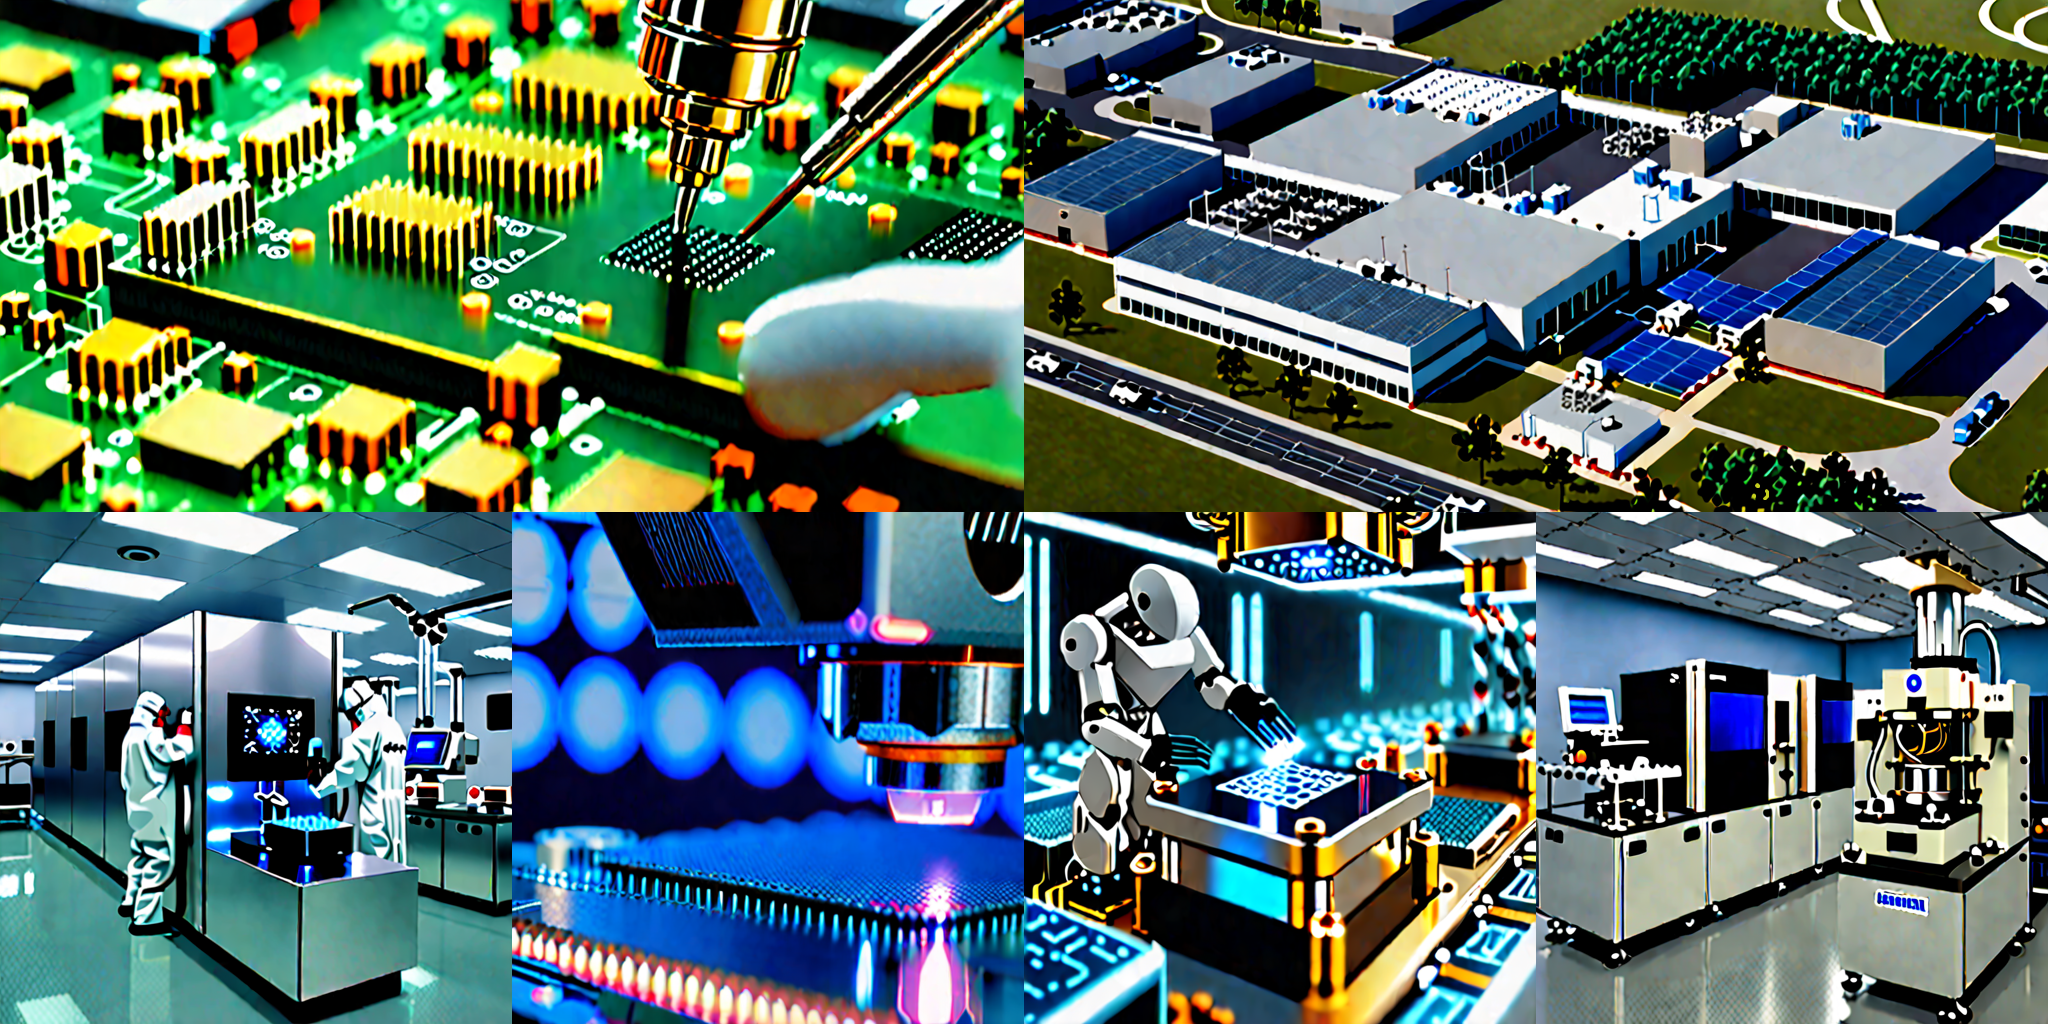
\includegraphics[width=1\linewidth]{collage.png}
\caption{Collage of AI-generated images for use in a themed
scenario}\label{fig:artifact-image-example}
\end{figure}

Finally, we noted that the Data Leakage Case lacks background email
conversations. Email conversations as part of a scenario can be divided
into three categories:

\begin{itemize}
\tightlist
\item
  Emails that are relevant to the focus or topic of the scenario, such
  as corporate espionage
\item
  Emails that are irrelevant to the scenario but are consistent with the
  persona included as part of the scenario, such as benign emails to
  coworkers
\item
  Emails wholly irrelevant to the scenario, such as marketing or spam
  emails
\end{itemize}

To generate these emails, DeepSeek-R1 was prompted to generate email
conversations according to the three email categories above in a
well-structured format that could easily be converted to a valid
\passthrough{\lstinline!.eml!} file using the Python standard library.
DeepSeek-R1 was provided details such as the email address to use when
sending/receiving emails and the corporate email domain to use in
relevant emails. An excerpt of a sample email conversation can be seen
in \autoref{fig:artifact-email-example}.

\begin{figure}[htbp]
\centering
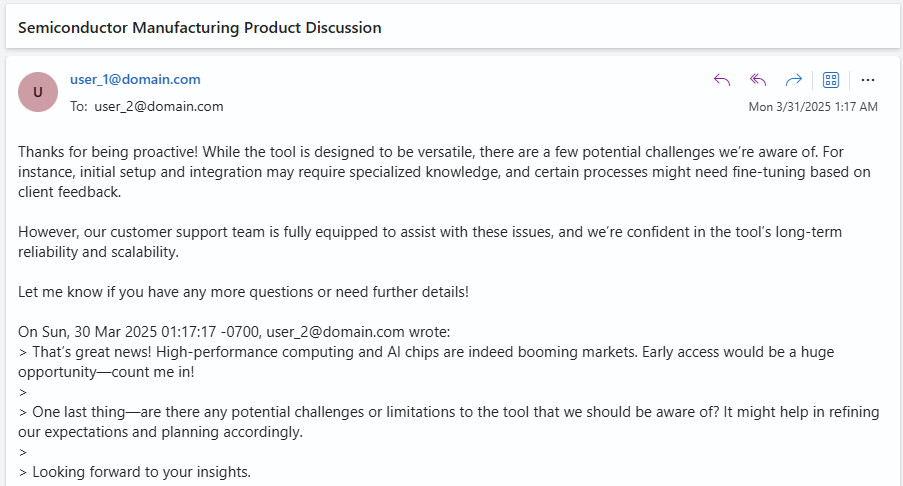
\includegraphics[width=1\linewidth]{email_snippet.png}
\caption{Sample of an AI-generated email
conversation}\label{fig:artifact-email-example}
\end{figure}

Consistent with the architectural diagram depicted in
\autoref{fig:architecture-full-a}, the use of generative AI in AKF is
almost entirely decoupled from other parts of the framework and can be
applied outside of synthesizer contexts. Although the three-step process
to generate the artifacts above was carried out manually, the same
process could be implemented in standalone modules in the AKF library.
There are various libraries and solutions for interfacing with Ollama
and ComfyUI through Python; these libraries could be leveraged in such
an implementation.

\section{Using LLMs for high-level
scenarios}\label{using-llms-for-high-level-scenarios}

The prior section addressed the challenge of generating individual
artifacts for a dataset. However, there remains the challenge of using
these artifacts to generate a cohesive scenario. That is, with an
overall scenario theme or goal in mind, what specific synthesizer
actions should be taken to construct a dataset that adheres to that
theme? Even with the automation routines provided by AKF and individual
artifacts prepared (whether created manually or using generative AI), it
still takes time to define a scenario, especially one that involves many
different types of actions that cannot easily be simplified into a small
number of synthesizer actions. This is true even with a simplified
declarative syntax.

One solution is to provide the details of AKF's declarative syntax to an
LLM and instruct it to generate valid declarative scripts. In
particular, there are two features of the declarative syntax that lends
itself well to this process:

\begin{itemize}
\tightlist
\item
  The role of each module is well-defined and corresponds one-to-one to
  a specific action that a human might take, such as visiting a set of
  websites.
\item
  The expected inputs for each module are well-defined, as they are
  documented by the required Pydantic argument model for each module.
\end{itemize}

To explore this, an instance of
\passthrough{\lstinline!deepseek-r1:32b!} was provided with the
following information. (The actual prompts and outputs used to derive
the content in this section are included with the scenario examples for
the AKF Windows agent.)

\begin{itemize}
\tightlist
\item
  An overview of the purpose of the declarative syntax.
\item
  The overall structure of the syntax, such as the required top-level
  keys and the structure of individual actions under the
  \passthrough{\lstinline!actions!} key.
\item
  A Markdown-formatted table in which each row contains the name,
  description, and arguments of available modules. Except for the
  arguments column, the table was equivalent to
  \autoref{tbl:akf-declarative-modules}.
\item
  A prompt delimited by \passthrough{\lstinline!<scenario\_prompt>!}
  tags that should be used to build the overall scenario.
\end{itemize}

We observed that this information was generally sufficient for
DeepSeek-R1 to ``understand'' the AKF syntax, allowing it to generate
simple declarative scripts. Although the prompt containing this
information was manually written, much of the prompt could be used as a
template and substituted with the contents of automatically generated
documentation. For example, the table of available modules could be
generated through existing code metadata, such as the contents of
docstrings and Pydantic argument models.

In one notable case, DeepSeek-R1 was directed to create a simple
scenario where a user visited news-related websites with Microsoft Edge
and entertainment-related websites with Google Chrome, ensuring that the
machine went through multiple power cycles throughout the scenario.
Although DeepSeek-R1 was not provided with examples specific to invoking
the \passthrough{\lstinline!chromium\_visit\_urls!} module, it correctly
constructed an argument dictionary containing several thematically
consistent websites for both browsers. Additionally, it correctly used
the \passthrough{\lstinline!vbox\_start\_machine!} and
\passthrough{\lstinline!vbox\_stop\_machine!} actions to perform
multiple power cycles.

However, DeepSeek-R1 struggled to understand the interactions between
related modules without additional guidance. For example, it did not
infer that the use of the \passthrough{\lstinline!vbox\_stop\_machine!}
and \passthrough{\lstinline!vbox\_start\_machine!} actions required that
a hypervisor instance had been previously created using
\passthrough{\lstinline!vbox\_start!}. Even when the module descriptions
were modified to state these requirements explicitly, it continued to
invoke \passthrough{\lstinline!vbox\_start\_machine!} without a
preceding \passthrough{\lstinline!vbox\_start!} action. In contrast,
DeepSeek-R1 appeared to understand that
\passthrough{\lstinline!chromium\_service\_start!} should be called
before calling any other Chromium-related modules, even when this
requirement was not stated. Indeed, the Chromium-related modules
support, but do not require, the use of
\passthrough{\lstinline!chromium\_service\_start!} to explicitly connect
to the Chromium RPyC subservice.

Additionally, DeepSeek-R1 would sometimes invoke modules incorrectly,
such as providing arguments that did not exist or invoking them with the
incorrect name. One notable example was that it incorrectly used
\passthrough{\lstinline!vbox\_start\_machine!} to both start and stop
the virtual machine, adding an erroneous
\passthrough{\lstinline!action: "stop"!} argument when stopping the
virtual machine. In some cases, DeepSeek-R1 deviated significantly from
the declarative syntax and used keys that did not exist, such as
specifying module arguments outside of the
\passthrough{\lstinline!args!} dictionary.

Despite these issues related to correctness, it was clear that
DeepSeek-R1 could convert abstract prompts into a sequence of actions
based on the available modules provided. Much like using declarative
scripts as a starting point for imperative scripts, these outputs can
likely be used as a starting point for more complex declarative scripts.
Furthermore, these issues could be alleviated by improving the details
of the prompt, such as providing specific examples of module usage and
the overall results they cause. In particular, DeepSeek-R1 is a
reasoning model, which means that it ``thinks out loud'' before
responding; the model's thoughts could be used to identify and eliminate
vagueness or uncertainty in the provided prompt. Writing precise,
detailed documentation with this LLM-oriented pipeline in mind could
further improve the quality of generated outputs.

As more declarative modules and functionality are added to AKF, it is
clear that LLMs can significantly accelerate converting abstract
scenario goals into a script that will carry out the necessary actions
to fulfill these goals. This is especially true given continuing
advancements in generative AI, which are likely to improve the
performance of these models in adhering to specific instructions.
